% TU Delft beamer template
% Author: Erwin Walraven (initial version was created by Maarten Abbink)
% Delft Universiy of Technology

\documentclass{beamer}
\usepackage[english]{babel}
\usepackage{calc}
\usepackage[absolute,overlay]{textpos}
\usepackage{graphicx}
\usepackage{subcaption}
\usepackage{amsmath}
\usepackage{amsfonts}
\usepackage{amsthm}
\usepackage{mathtools}
\usepackage{comment}
\usepackage{MnSymbol,wasysym}

\setbeamertemplate{navigation symbols}{} % remove navigation symbols
\mode<presentation>{\usetheme{tud}}

% BIB SETTINGS
%\usepackage[backend=bibtex,firstinits=true,maxnames=30,maxcitenames=20,url=false,style=authoryear]{biblatex}
%\bibliography{bibfile}
%\setlength\bibitemsep{0.3cm} % space between entries in the reference list
%\renewcommand{\bibfont}{\normalfont\scriptsize}
%\setbeamerfont{footnote}{size=\tiny}
%\renewcommand{\cite}[1]{\footnote<.->[frame]{\fullcite{#1}}}


\title[]{Transiently-powered Battery-free Robot}
\institute[]{Delft University of Technology, The Netherlands}
\author{Koen Schaper}
%\date{}

\logo{
\includegraphics[width=3cm]{pics/es_logo_cyan_black_rgb}}

\begin{document}
{
\setbeamertemplate{footline}{\usebeamertemplate*{minimal footline}}
\frame{\titlepage}
}

{\setbeamertemplate{footline}{\usebeamertemplate*{minimal footline}}

}

\begin{frame}{Example frame 1}
This is the first frame
\end{frame}

\begin{frame}{Overview}
	\begin{itemize}
		\item item 1
		\item Conclusion
		\item 
	\end{itemize}
\end{frame}

\begin{frame}{Schematic overview}
	\begin{center}
		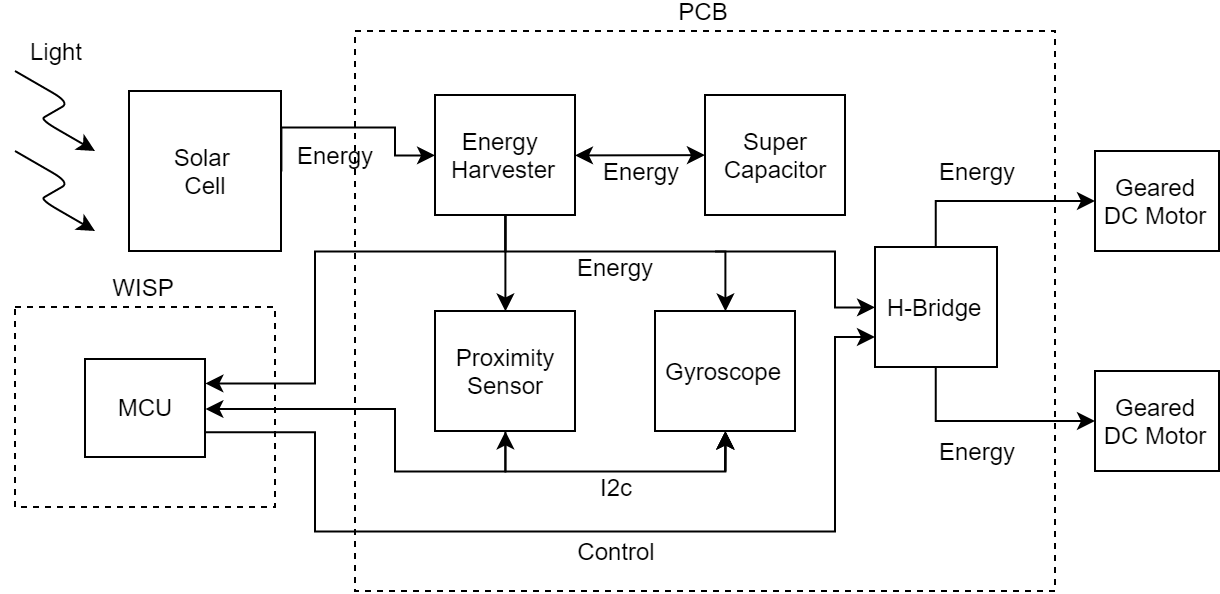
\includegraphics[width=0.9\textwidth]{pics/schematic_robot_v2.png}
	\end{center}
\end{frame}

\begin{frame}{Robot implementation}
	\begin{center}
		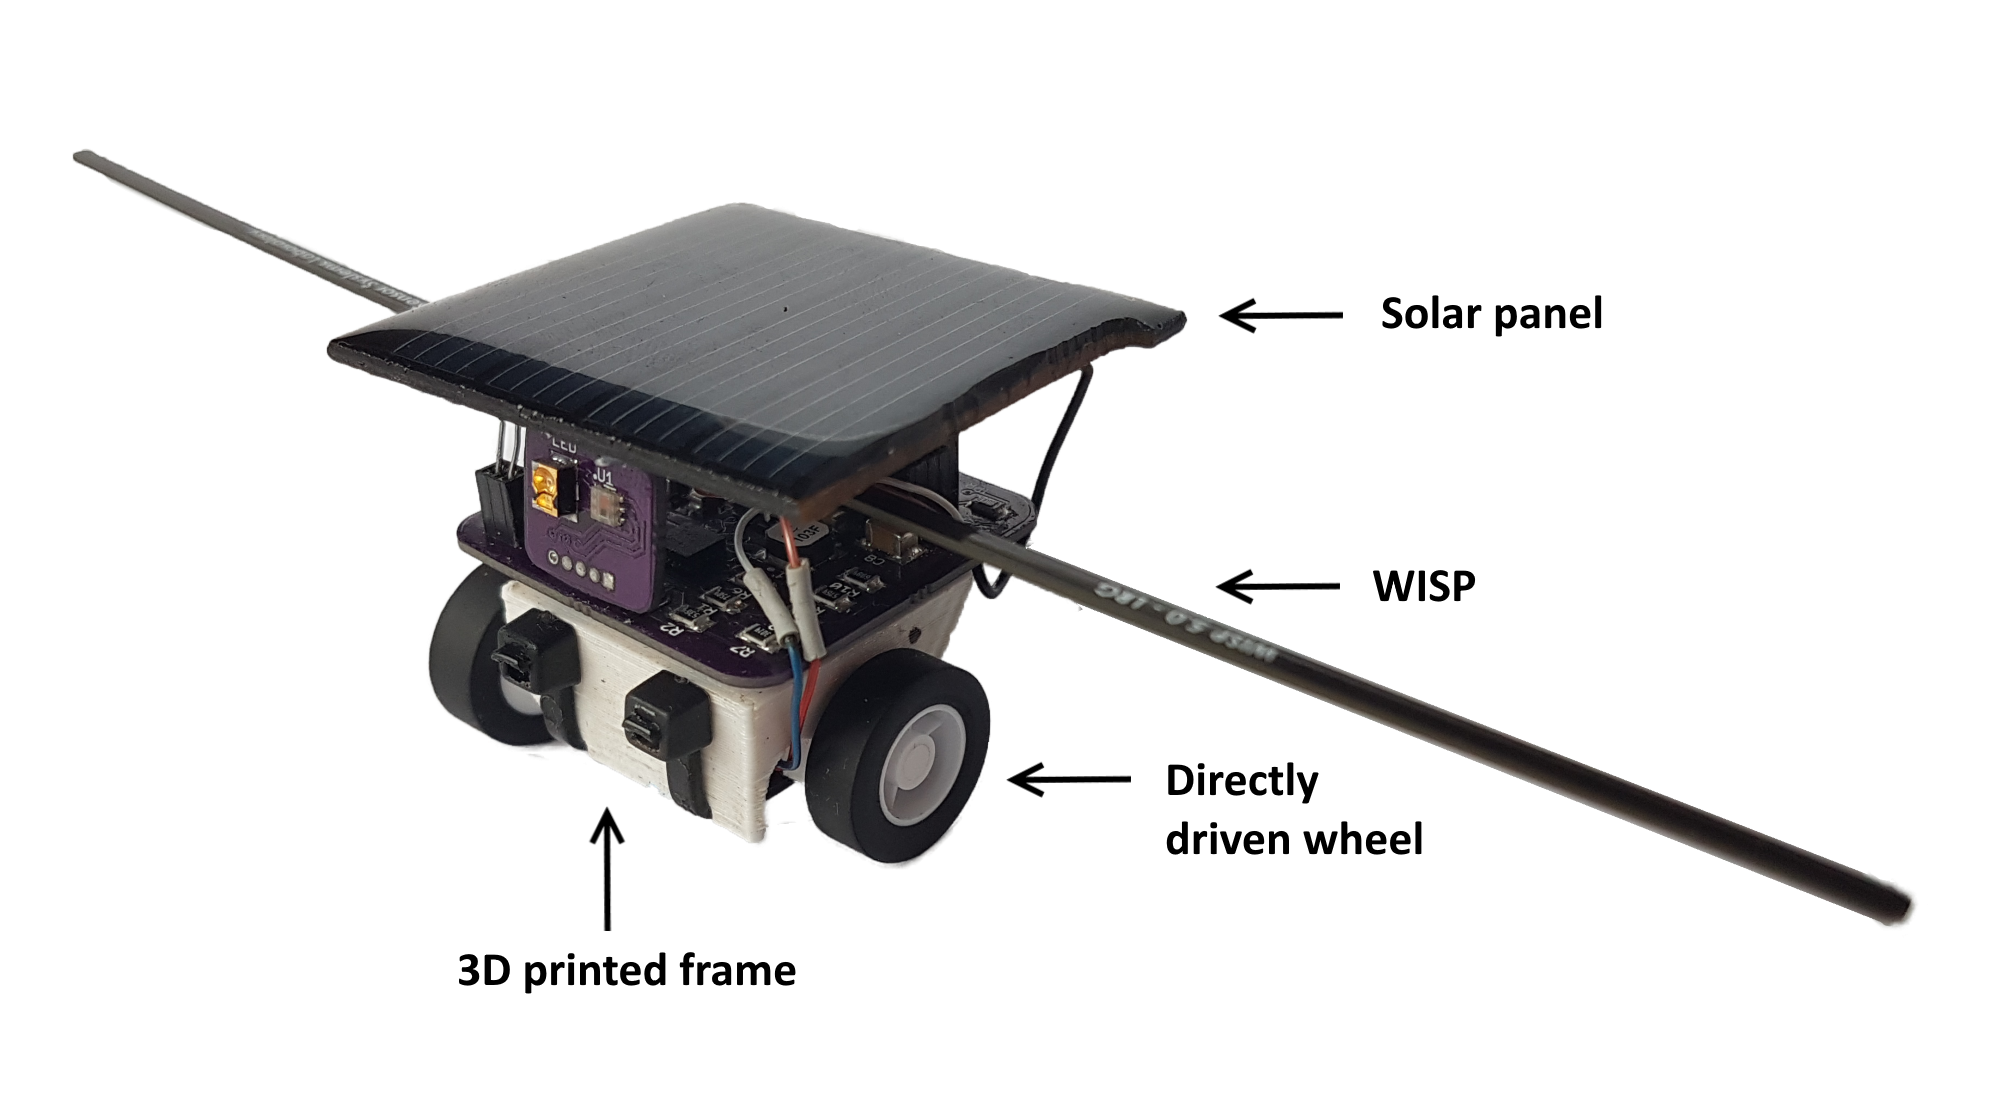
\includegraphics[width=0.9\textwidth]{pics/tp_robot2.png}
	\end{center}
\end{frame}

\begin{frame}{Control loop}
	\begin{center}
		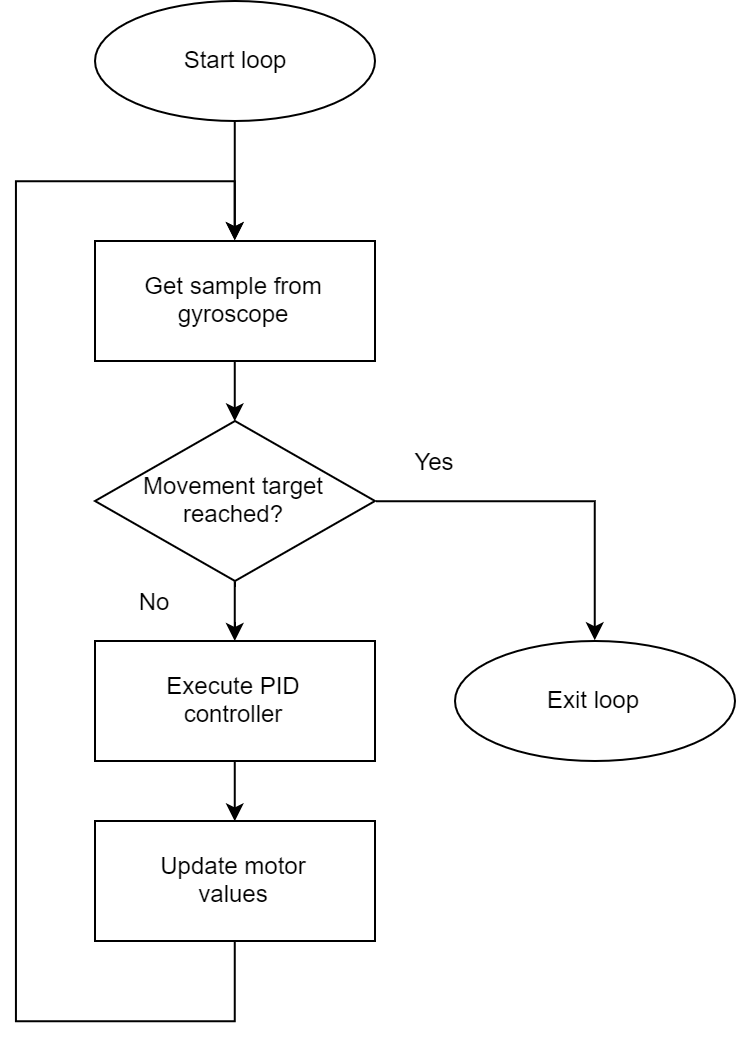
\includegraphics[width=0.4\textwidth]{pics/Flowchart_code.png}
	\end{center}
\end{frame}

\begin{frame}{Tuning PID controller}
	\begin{figure}
		\begin{center}
		\begin{subfigure}[b]{0.49\textwidth}
			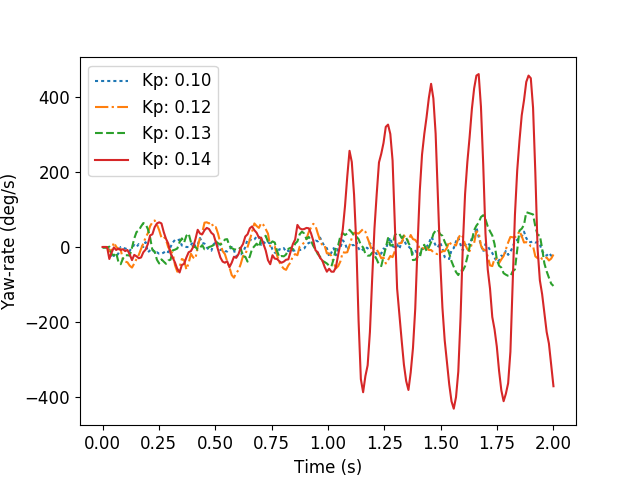
\includegraphics[width=\textwidth]{pics/straight_ku.png}
			\caption*{Determining the ultimate gain}
		\end{subfigure}
		\begin{subfigure}[b]{0.49\textwidth}
			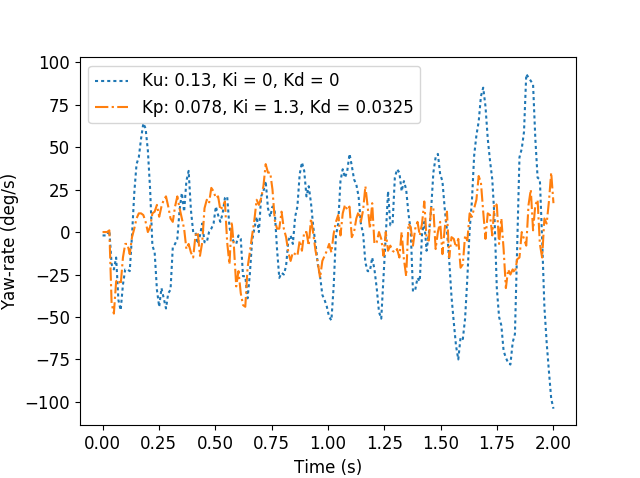
\includegraphics[width=\textwidth]{pics/straight_ku_with_tu.png}
			\caption*{Result of applying the gains}
		\end{subfigure}
		\end{center}
	\end{figure}
\end{frame}

\begin{frame}{Evaluation}
	\vspace{1em}
	\begin{figure}
		\centering
		\begin{subfigure}[b]{0.45\textwidth}
			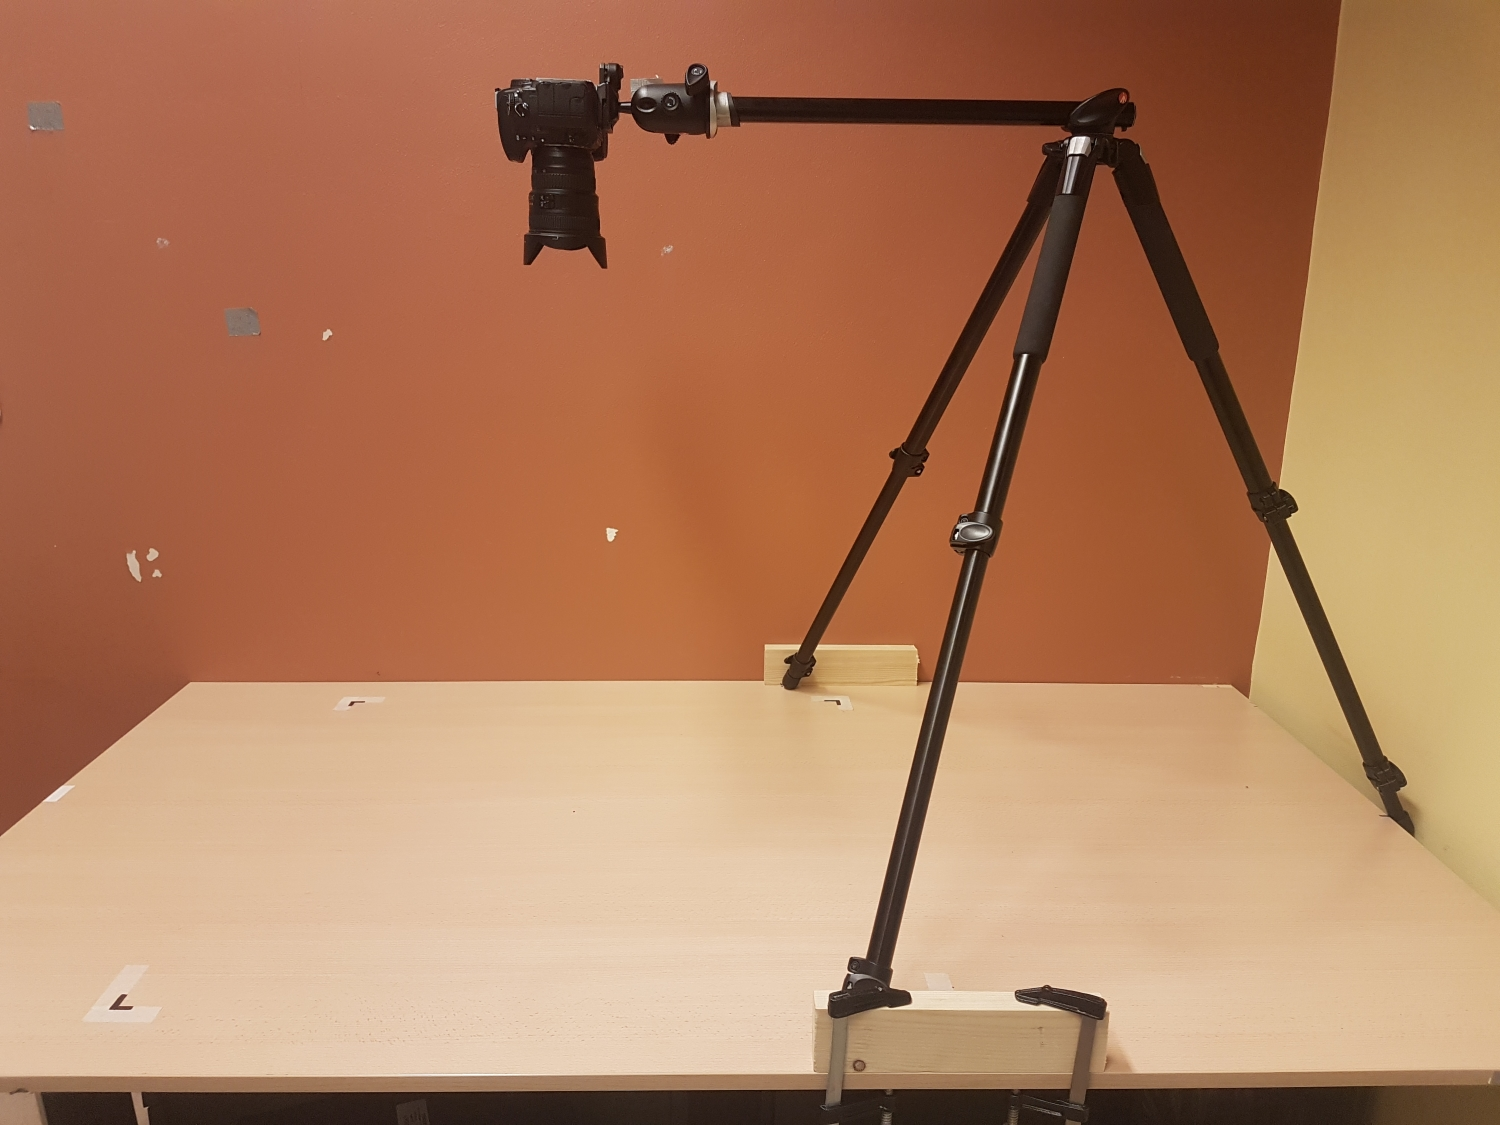
\includegraphics[width=\textwidth]{pics/movement_setup.jpg}
			\caption*{Camera setup}
		\end{subfigure}
		\quad
		\begin{subfigure}[b]{0.45\textwidth}
			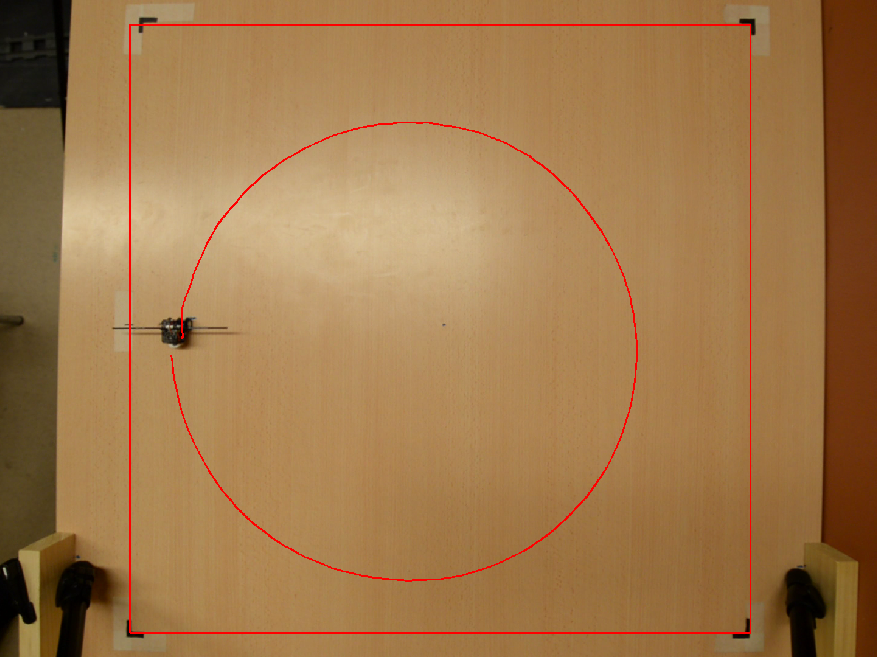
\includegraphics[width=\textwidth]{pics/movement_example.png}
			\caption*{Tracking with OpenCV}
		\end{subfigure}
	\end{figure}
\end{frame}

\begin{frame}{Minimum on time}
	\begin{figure}
		\centering
		\begin{subfigure}[b]{0.32\textwidth}
			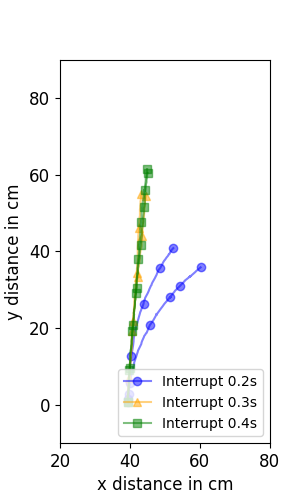
\includegraphics[width=\textwidth]{pics/figure_40.png}
			\caption*{Duty cycle 40\%}
		\end{subfigure}
		\hspace{2em}
		\begin{subfigure}[b]{0.32\textwidth}
			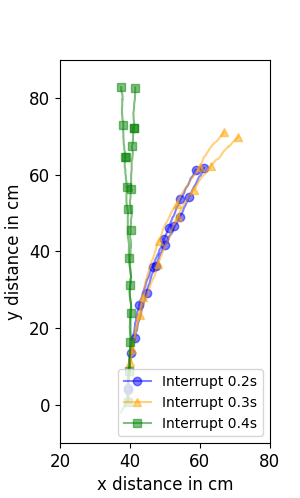
\includegraphics[width=\textwidth]{pics/figure_90.png}
			\caption*{Duty cycle 90\%}
		\end{subfigure}
	\end{figure}
\end{frame}

\begin{frame}{Straight movements}
	\begin{figure}
		\centering
		\begin{subfigure}[b]{0.32\textwidth}
			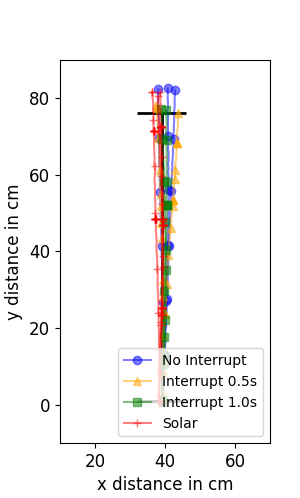
\includegraphics[width=\textwidth]{pics/straight_40.png}
			\caption*{Duty cycle 40\%}
		\end{subfigure}
		\hspace{2em}
		\begin{subfigure}[b]{0.32\textwidth}
			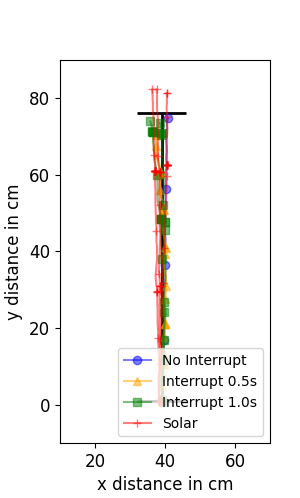
\includegraphics[width=\textwidth]{pics/straight_90.png}
			\caption*{Duty cycle 90\%}
		\end{subfigure}
	\end{figure}
\end{frame}

\begin{frame}{Circular movements}
	\begin{figure}[h!]
		\centering
		\begin{subfigure}[b]{0.49\textwidth}
			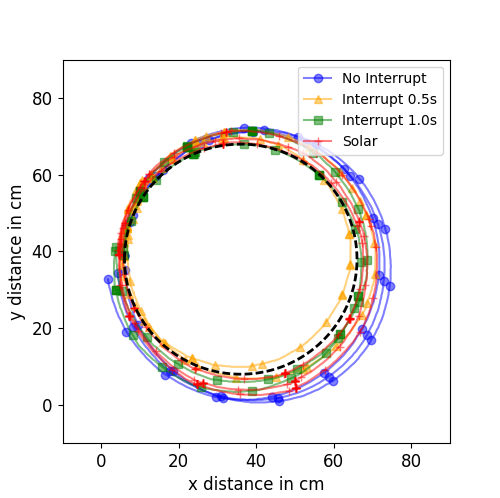
\includegraphics[width=\textwidth]{pics/circle_40.png}
			\caption*{Duty cycle 40\%}
		\end{subfigure}
		\begin{subfigure}[b]{0.49\textwidth}
			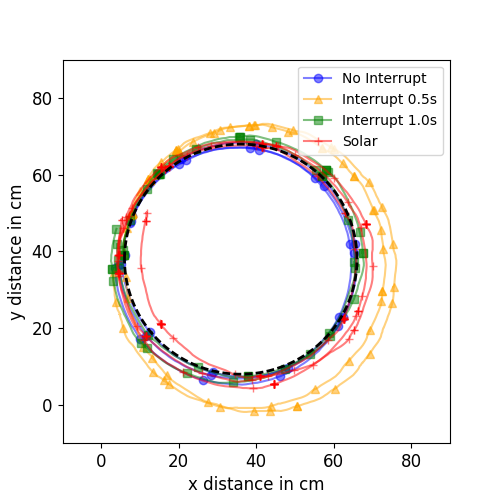
\includegraphics[width=\textwidth]{pics/circle_90.png}
			\caption*{Duty cycle 90\%}
		\end{subfigure}
	\end{figure}
\end{frame}

\begin{frame}{Conclusion}
	\begin{itemize}
		\item item 1
		\item item 2
	\end{itemize}
\end{frame}

\begin{frame}{Future Work}
	\begin{itemize}
		\setlength\itemsep{1em}
		\item Speed feedback 
		\item Communication
		\item Transiently-powered swarm
		\item Size reduction
		\item Sensing capabilities
	\end{itemize}
\end{frame}

\end{document}
